\documentclass[10pt,aspectratio=169]{beamer}
\usetheme{Boadilla}
\usecolortheme{dove}
\usepackage[T1]{fontenc}
\usepackage{lmodern,amsmath,amssymb,booktabs,array,tikz,graphicx,xcolor}
\usetikzlibrary{arrows.meta,positioning,calc}
\setbeamertemplate{navigation symbols}{}
\setbeamertemplate{itemize items}[circle]
\setbeamersize{text margin left=7mm,text margin right=7mm}
\definecolor{navy}{HTML}{18334C}
\definecolor{teal}{HTML}{17816D}
\definecolor{blue}{HTML}{456EA8}
\definecolor{ochre}{HTML}{B47A22}
\definecolor{red}{HTML}{B95643}
\definecolor{soft}{HTML}{F3F5F6}
\setbeamercolor{structure}{fg=navy}
\setbeamercolor{frametitle}{fg=navy}
\setbeamercolor{title}{fg=navy}
\setbeamertemplate{footline}{\hspace{7mm}\scriptsize Reference-crystal selection for Crys-JEPA\hfill\insertframenumber/\inserttotalframenumber\hspace{7mm}\vspace{3mm}}
\graphicspath{{../assets/}}
\newcommand{\ehull}{E_{\mathrm{hull}}}
\newcommand{\source}[1]{\par\vspace{1mm}{\scriptsize\color{gray}#1}}
\tikzset{stage/.style={draw=navy,line width=.5pt,rounded corners=1mm,align=center,font=\small,minimum height=9mm,inner sep=2mm},arr/.style={-{Stealth[length=1.5mm]},line width=.6pt,draw=navy}}
\title{Reference-crystal selection for Crys-JEPA}
% \subtitle{}
\author{Group 2 Project Progress Report}
\institute{}
\date{October 30, 2026}
\begin{document}

\begin{frame}
\titlepage
\vspace{-5mm}
\begin{center}
    %\small
% Known MP20 crystals provide the reference bank. Generated crystals are screened with MatterSim.\\[2mm]
Reports of the completed baselines and GNN evaluation.
\end{center}
\end{frame}

\begin{frame}{Motivation}
\begin{itemize}\setlength\itemsep{4mm}
\item Diffusion models generate many candidate crystals.
\item Crys-JEPA ranks candidates by their similarity to known reference crystals.
\item The reference choice controls which candidates enter the expensive refinement loop.
\item A useful reference set should capture structural context and improve the number of stable candidates selected at a fixed budget.
\end{itemize}
\vspace{4mm}
\centering
\resizebox{.90\linewidth}{!}{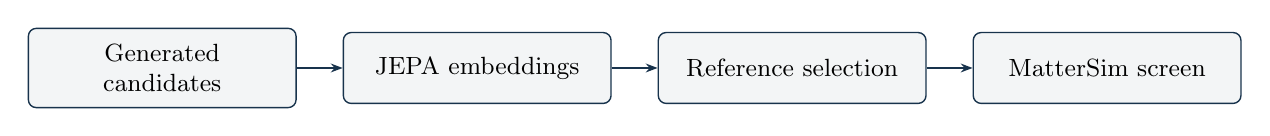
\begin{tikzpicture}
\node[stage,fill=soft,text width=30mm] (gen) at (0,0) {Generated candidates};
\node[stage,fill=soft,text width=30mm] (emb) at (4,0) {JEPA embeddings};
\node[stage,fill=soft,text width=30mm] (ref) at (8,0) {Reference selection};
\node[stage,fill=soft,text width=30mm] (eval) at (12,0) {MatterSim screen};
\draw[arr] (gen)--(emb);\draw[arr] (emb)--(ref);\draw[arr] (ref)--(eval);
\end{tikzpicture}
}
\source{Crys-JEPA uses a known-crystal reference bank and a fixed candidate-selection budget.}
\end{frame}

\begin{frame}{Existing Crys-JEPA pipeline}
\centering
\vspace{5mm}
\includegraphics[width=.90\linewidth]{pipeline_diagram.pdf}
\vspace{1mm}
\begin{itemize}
\item References come from 27,136 known MP20 training crystals.
\item Generated candidates are used as queries to pick the top K references.
\item A candidate passes the current screen when corrected MatterSim energy above the fixed hull is at most $0.1$ eV/atom.
\end{itemize}
\source{MatterSim is a comparative ML potential screen. It is not a DFT confirmation.}
\end{frame}

\begin{frame}{Original reference score}
For a candidate $c$, collect known references whose elements are contained in the candidate system:
\[
R(c)=\{r\in\mathcal D_{\mathrm{MP20}}:\operatorname{elements}(r)\subseteq\operatorname{elements}(c)\}.
\]
The original score is
\[
s(c)=\frac{1}{|R(c)|}\sum_{r\in R(c)}\lVert h_c-h_r\rVert_2^2.
\]
\begin{itemize}\setlength\itemsep{3mm}
\item Smaller scores rank first.
\item Every reference structure receives equal weight.
\item Different polymorphs of one formula remain separate structures.
\item We define: A chemical system is a set of elements. A reference subsystem is a known crystal whose elements are a subset of that system.
\end{itemize}
\end{frame}

\begin{frame}{Why a chemical subsystem alone may miss useful structure}
\begin{columns}[T]
\column{.48\textwidth}
\begin{itemize}\setlength\itemsep{3mm}
\item A polymorph is a different crystal structure with the same formula.
\item For Na, the MP20 bank contains several space groups and different energies.
\item A formula-only view groups these structures by chemistry, but it does not describe their structural differences.
\item A candidate may be close to a useful structure even when its best chemical match is outside the exact subsystem.
\end{itemize}
\column{.48\textwidth}
\begin{center}
{\scriptsize\begin{tabular}{lccc}
\toprule
Material & Formula & $E_{\rm hull}$ & Space group\\
\midrule
mp-1186040 & Na & 0.0179 & 223\\
mp-567772 & Na & 0.0130 & 220\\
mp-1186055 & Na & 0.0248 & 213\\
mp-973198 & Na & 0.0079 & 166\\
mp-127 & Na & 0.0123 & 229\\
\bottomrule
\end{tabular}}
\end{center}
\vspace{1mm}
{\scriptsize\textit{Example from the MP20 polymorph inspection shared by the group.}}\par
\vspace{2mm}
\noindent\small Same chemistry does not mean the same structure or the same energy.
\end{columns}
\end{frame}

\begin{frame}{ Comparing the candidate selection from these methods}
\begin{columns}[T]
\column{.30\textwidth}
\textbf{Shared set}
\small Candidates selected by both the original Crys-JEPA rule and the new rule. These candidates do not explain the difference.
\column{.30\textwidth}
\textbf{Added set}
\small Candidates selected by the new rule but missed by the original rule. These are the extra candidates we study.
\column{.30\textwidth}
\textbf{Removed set}
\small Candidates selected by the original rule but missed by the new rule. These are the candidates traded away.
\end{columns}
\vspace{7mm}
\centering
\begin{tabular}{lrr}
\toprule
Group & Count & MatterSim pass rate \\
\midrule
Shared & 455 & 37\% \\
Added & 1,394 & 44\% \\
Removed & 1,394 & 34\% \\
\bottomrule
\end{tabular}
\end{frame}

\begin{frame}{Observed selection change}
\begin{columns}[T]
\column{.62\textwidth}
\centering
\includegraphics[height=.19\textheight,viewport=0 288 396 576,clip]{selection_explanation.png}\\[-1mm]
\includegraphics[height=.19\textheight,viewport=396 288 792 576,clip]{selection_explanation.png}\\[-1mm]
\includegraphics[height=.19\textheight,viewport=0 0 396 288,clip]{selection_explanation.png}
\column{.35\textwidth}
\scriptsize
\textbf{Panel A: selected-set change.} The new rule adds 613 candidates and removes 475 relative to the shared set.\\[2mm]
\textbf{Panel B: nearest-reference angle.} Added candidates have a close known reference, often inside the 1 degree gate.\\[2mm]
\textbf{Panel C: local versus pool score.} A close neighbour does not always give a low mean distance to the full chemical pool. The plot shows why a local-neighbour rule can select different candidates from the original mean-distance rule.
\end{columns}
\end{frame}

\begin{frame}{Experiments}
\centering
\vfill
{\Huge\color{navy}Experiments}
\vfill
\end{frame}

\begin{frame}{Baseline methods}
\begin{tabular}{>{\raggedright\arraybackslash}p{.29\textwidth}p{.62\textwidth}}
\toprule
Baseline & Definition\\
\midrule
Original Crys-JEPA & Mean squared JEPA distance over eligible known MP20 references.\\[2mm]
Cosine KNN, $k=5$ & Use the five closest known references by cosine distance.\\[2mm]
Intersection KNN & Use the overlap between the original pool and cosine neighbours \\[2mm]
Formula-balanced mean & Reduce the effect of formulas with many polymorphs.\\[2mm]
Random references & Use a matched random reference pool as a negative control.\\
\bottomrule
\end{tabular}
\vspace{5mm}
\end{frame}

\begin{frame}{Baseline results at the 5\% budget}
\centering
\begin{tabular}{lrrr}
\toprule
Method & Passes & Yield & $\Delta$ vs original \\
\midrule
Original Crys-JEPA & 721 & 40.8\% & -- \\
Cosine KNN & 722 & 40.9\% & \textcolor{teal}{+1\;(+0.1\,pp)} \\
Intersection KNN & 760 & 43.0\% & \textcolor{teal}{+39\;(+2.2\,pp)} \\
Formula prior & 693 & 39.2\% & \textcolor{red}{-28\;(-1.6\,pp)} \\
Random references & 679 & 38.4\% & \textcolor{red}{-42\;(-2.4\,pp)} \\
\bottomrule
\end{tabular}
\vspace{6mm}
\begin{itemize}
\item Intersection KNN is the strongest simple baseline.
\item It combines chemical eligibility with the five nearest JEPA references.
\item We rank candidates first, then evaluate the selected candidates with MatterSim.
\end{itemize}
\source{MatterSim pass means corrected energy above the fixed hull is at most $0.1$ eV/atom.}
\end{frame}

\begin{frame}{Graph model setup}
\begin{columns}[T]
\column{.31\textwidth}
\textbf{Nodes}
\begin{itemize}\setlength\itemsep{2mm}
\item Each node is one known MP20 reference crystal.
\item The node stores its frozen 512-D JEPA embedding.
\item Composition fractions describe the elements in the crystal.
\end{itemize}
\column{.31\textwidth}
\textbf{Edges}
\begin{itemize}\setlength\itemsep{2mm}
\item Connect each reference to its ten nearest references by cosine distance.
\item Add the reverse edge so the graph is symmetric.
\item Store cosine distance, raw squared distance, and chemical eligibility.
\end{itemize}
\column{.31\textwidth}
\textbf{Prediction}
\begin{itemize}\setlength\itemsep{2mm}
\item A generated candidate enters as a query, never as a graph node.
\item Message passing updates each known reference using its neighbours.
\item A candidate-conditioned readout scores the reference set and predicts a MatterSim pass.
\end{itemize}
\end{columns}
\vspace{3mm}
\centering\small
The KNN graph defines who can exchange information. The edge features and candidate-conditioned readout decide how that information affects the final score.
\end{frame}

\begin{frame}{Models compared}
\begin{tabular}{>{\raggedright\arraybackslash}p{.23\textwidth}p{.68\textwidth}}
\toprule
Model & Message-passing rule\\
\midrule
GCN & Mix each reference with its neighbouring reference states using degree normalization, then update the node representation.\\[3mm]
GraphSAGE & Compute a mean summary of neighbouring reference states and combine it with the current reference state.\\[3mm]
GAT & Learn a separate importance weight for each neighbour before updating the reference representation.\\[3mm]
\bottomrule
\end{tabular}
\vspace{6mm}
\end{frame}

\begin{frame}{Results across selection budgets}
\centering
{\scriptsize\begin{tabular}{lrrrr}
\toprule
Method & 1\% & 2\% & 5\% & 7\% \\
\midrule
Original Crys-JEPA & 189 & 328 & 721 & 954 \\
Cosine KNN & 175\;\textcolor{red}{(-14)} & 318\;\textcolor{red}{(-10)} & 722\;\textcolor{teal}{(+1)} & 950\;\textcolor{red}{(-4)} \\
Intersection KNN & 186\;\textcolor{red}{(-3)} & 333\;\textcolor{teal}{(+5)} & 760\;\textcolor{teal}{(+39)} & 1,013\;\textcolor{teal}{(+59)} \\
Angle gate & 193\;\textcolor{teal}{(+4)} & 348\;\textcolor{teal}{(+20)} & 769\;\textcolor{teal}{(+48)} & 1,042\;\textcolor{teal}{(+88)} \\
\midrule
GCN & 188\;\textcolor{red}{(-1)} & 333\;\textcolor{teal}{(+5)} & \textbf{774}\;\textcolor{teal}{(+53)} & \textbf{1,067}\;\textcolor{teal}{(+113)} \\
GAT & 175\;\textcolor{red}{(-14)} & 329\;\textcolor{teal}{(+1)} & 745\;\textcolor{teal}{(+24)} & 1,022\;\textcolor{teal}{(+68)} \\
GraphSAGE & 183\;\textcolor{red}{(-6)} & 325\;\textcolor{red}{(-3)} & 745\;\textcolor{teal}{(+24)} & 1,018\;\textcolor{teal}{(+64)} \\
\bottomrule
\end{tabular}}
\vspace{5mm}
\begin{itemize}\setlength\itemsep{2mm}
\item At 5\%, GCN selects 774 MatterSim passes versus 721 for Crys-JEPA.
\item At 7\%, GCN selects 1,067 passes versus 954 for Crys-JEPA.
\item The table shows the best observed run for each model family at each budget. Seed details stay in the raw result files.
\end{itemize}
\source{Counts are unique selected candidates passing the MatterSim hull screen.}
\end{frame}

\begin{frame}{What the current results mean}
\begin{itemize}\setlength\itemsep{4mm}
\item The angle gate and KNN controls change which chemical systems receive selection slots.
\item Same-chemistry controls remove most of the earlier global gain.
\item Same-formula pair accuracy is close to 50\%, so the current score does not strongly order polymorphs by stability.
\item The completed cluster evaluation shows a positive graph-model result at the fixed 5\% budget.
\item The result is a MatterSim screening comparison. It does not prove lower true formation energy.
\end{itemize}
\end{frame}

\begin{frame}{Current evidence and limits}
\begin{itemize}\setlength\itemsep{4mm}
\item The reference bank is known MP20 training data.
\item MatterSim labels provide a consistent comparative screen.
\item The current gains are screening-yield gains, not proof of lower true formation energy.
\item We still need to analyse the results of individual success/reject cases and understand at a deeper level.
\end{itemize}
\vspace{4mm}
\centering\large\color{navy}Reference quality must be tested by downstream candidate.
\end{frame}

\end{document}
